\chapter{Разработка принципов создания специального математического и алгоритмического обеспечения проектирования архитектуры  }\label{ch:ch3}
\section{Разработка принципов создания специального математического и алгоритмического обеспечения проектирования архитектуры  }\label{ch:ch3/sec1}

Основным принципом создания системы поддержки принятия решений назовем модуль функциональной работы классификатора на основе нечеткой логики.
модель деревьев поиска закономерностей с нечеткой логикой должна аппроксимировать некоторый функционал в соответствии со следующими принципами:
\begin{enumerate}
    \item множество входных параметров переменных $X = {x_1, x_2, ..., x_n}$, характеризующие объект получения рекомендации,
    \item множество выходных переменных $Y = {y_1, y_2, ..., y_n}$, характеризуюших рекомендацию по объекту проектирования,
    \item множество лингвистических переменных термов $A = {a_j, a_{j+1}, a_m}$, которые являются мерой соотнесения с нечеткой функцией классификации переменных $x_i$,
    \item множество лингвистических переменных термов $B = {b_j, b_{j+1}, b_m}$, которые являются мерой соотнесения с нечеткой функцией классификации переменных $y_i$,
    \item функция принадлежности ~\cref{eq:equation45},
    \item матрица знаний, согласно Рисунку ~\cref{fig:KBase}.
\end{enumerate}


После принципа преобразования получаем следующую систему однородных нелинейных преобразований
\begin{equation}
    \label{eq:equation57}
     \left\{\begin{array}{ll} 
    y_1 = F_1(X,W,C,\Psi) \textrm{,} 
    \\ y_2 = F_2(X,W,C,\Psi)  \textrm{,}
    \\ ... 
     \\ y_n = F_n(X,W,C,\Psi) 
      & \end{array} \right. \]
\end{equation}

где $X = {x_1, x_2, ..., x_n}$ - вектор входный переменных, описывающих систему,

$W$ - вектор весовых коэффициентов продукционных правил,

$C,\Psi$ - вектор функций принадлежностей лингвистических термов.


Обучающая выборка задается в виде пары $(X^p, Y^p)$, принцип поиска эвристического процесса обучения может быть описани следущим образом:
\begin{equation}
    \label{eq:equation58}
    \begin{alignedat}{2}
        \sum_{p=1}^L[F_1(X^p,W,C,\Psi) - y_1^p]^2 + \\
        + \sum_{p=1}^L[F_1(X^p,W,C,\Psi) - y_2^p]^2 +  ... \\
       ... +  \sum_{p=1}^L[F_1(X^p,W,C,\Psi) - y_p^p]^2 = \\
        = \sum_{j = 1}^q{\sum_{p=1}^L{[F_j(X^p,W,C,\psi) - y^p_j]^2}}
        = min\{W,C,\Psi\}
    \end{alignedat}
\end{equation}

Принцип создания обучающей выборки состоит в том, чтобы предъявить факты и уже известный закономерный вывод для обучения, чтобы модель могла начать процесс апроксимации функционала соответствия, опираясь на эвристический поиск соответствия.
Принцип работы функциональной схемы обработки и формирования эвристического соответствия входному и выходному вектору переменных приведен на Рисунке ~\cref{fig:FL}
\begin{figure}[ht]
    \centerfloat{
        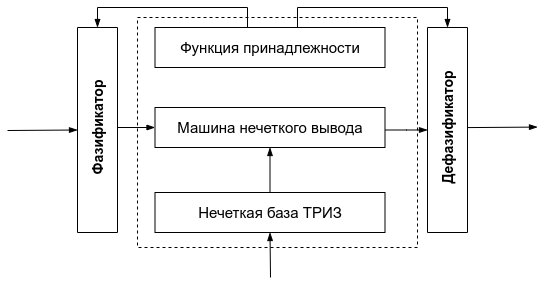
\includegraphics[scale=0.8]{Dissertation/images/DISSER-9.png}
    }
    \caption{Структура принципа преобразования}\label{fig:FL}
\end{figure}

Таким образом основным принципом формирования модели поддержки принятия решений является эвристический аппроксиматор функционала поиска закономерностей для вывода, т.е. функционала эвристического соответствия между входным вектором и выходным.

\subsection{Выбор основного принципа реализации модели}\label{subsec:ch3/sec2/sub1}

На Рисунке~\cref{fig:FLbase} представлен основной принцип реализации модели эвристического соответствия между входными переменными и выходными.
\begin{figure}[ht]
    \centerfloat{
        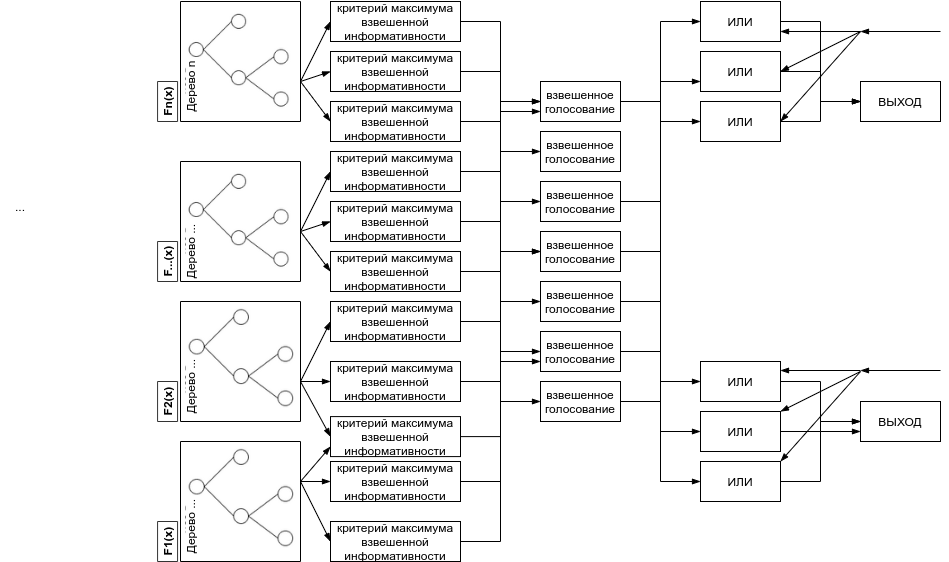
\includegraphics[scale=0.5]{Dissertation/images/DISSER-10.png}
    }
    \caption{Структура принципа формирования эвристического соответствия}\label{fig:FLbase}
\end{figure}

Структура основного принципа реализации модели состоит из следующих этапов:
\begin{enumerate}
    \item формирование данных для обучения,
    \item настройка нечетких функционалов принадлежности,
    \item обучение по соревнованию,
    \item удаление закономерностей, не прошедшие критерий максимума взвешенной информативности,
    \item комбинирование закономерностей согласно синтезу деревьев,
    \item финальная настройка соответствия нечетких функционалов и входных и выходных параметров на основе критерия максимума взвешенной информативности. 
\end{enumerate}

Настройка функционала принадлежности
\begin{equation}
    \label{eq:equation59}
     y_i^{k}(x) = e^{\frac{-(x_i-x_i)}{2\sigma_i^2}}
\end{equation}

Обучение по голосованию может быть представлено в виде
\begin{equation}
    \label{eq:equation60}
     \bigtriangleup c_\omega(t) = \eta(t)(x-c_\omega(t))
\end{equation}

где $\eta(t)$ - градиент обучения.

Шаг градиента выбирается произвольным образом, эвристически, затем исправляется в соответствии с откликом в виде ошибки обучения. Алгоритм голосования оценивает две матрицы весовых характеристик параметров важности фактов, а также качество связей между матрицами. В этом месте допускается использование и полноценного алгоритма нейронной сети, таких, как, например, генеративно-состязательные нейронные сети~\cite{Goodfellow}.
\begin{equation}
    \label{eq:equation61}
     \bigtriangleup \omega = y_j(y_j - \omega_{ji})
\end{equation}

Комбинирование правил выполняется с помощью поиска закономерностей, синтезу деревьев и взвешенного голосования. Окончательный этап формирования принципа соответствия строится на основании функции поправки ошибок критерия максимума взвешенной информативности
\begin{equation}
    \label{eq:equation62}
     e_t = (y_t - d_k)
\end{equation}

Таким образом, основным принципом формирования эвристического функционала принадлежности являются этапы формирования знаний и поправки градиента критерия максимума взвешенной информативности обучения с помощью возмущаеющего сигнала ошибки, это формирует функционал соответствия в виде нелинейной адаптивной комбинированной системы с возмущением. 
На Рисунке ~\cref{fig:FLmetrics} представлен основные принципы расчета расстояний. 
\begin{figure}[ht]
    \centerfloat{
        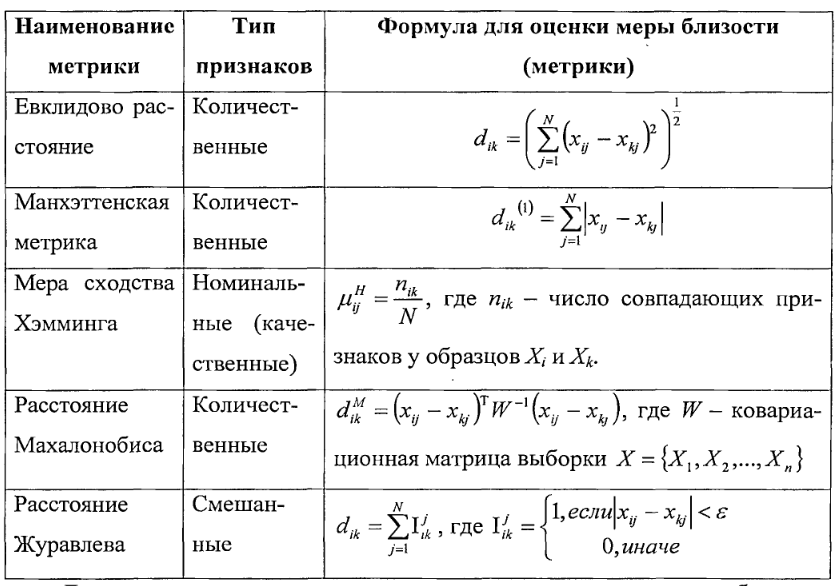
\includegraphics[scale=0.35]{Dissertation/images/DISSER-11.png}
    }
    \caption{Структура принципа расчета расстояния}\label{fig:FLmetrics}
\end{figure}

\subsection{Назначение специального математического и алгоритмического обеспечения}\label{subsec:ch3/sec2/sub1}
Назначение системы состоит в поддержки принятия решений на этапе проектирования архитектура программного обеспечения.

\section{Функциональные возможности программного обеспечения}\label{sec:ch3/sec3}

Функциональные возможности программного обеспечения на текущем этапе работ позволяет вводит в пользовательском режиме информацию о характеристиках планируемой архитектуры программного обеспечения и выводит рекомендованную структуру организации и необходимую инфраструктуру для проектирования. Система впоследствии может быть дополнена модулями анализа кода, а также модулями анализа отношений между сущностями и таблицами в базе данных.

\subsection{Ввод данных}\label{subsec:ch3/sec3/sub1}
Ввод данных происходит по заполнению специальной формы представленной на Рисунках~\cref{fig:ui-1,fig:ui-2,fig:ui-3,fig:ui-4,fig:ui-5,fig:ui-6}. 
\begin{figure}[ht]
    \centerfloat{
        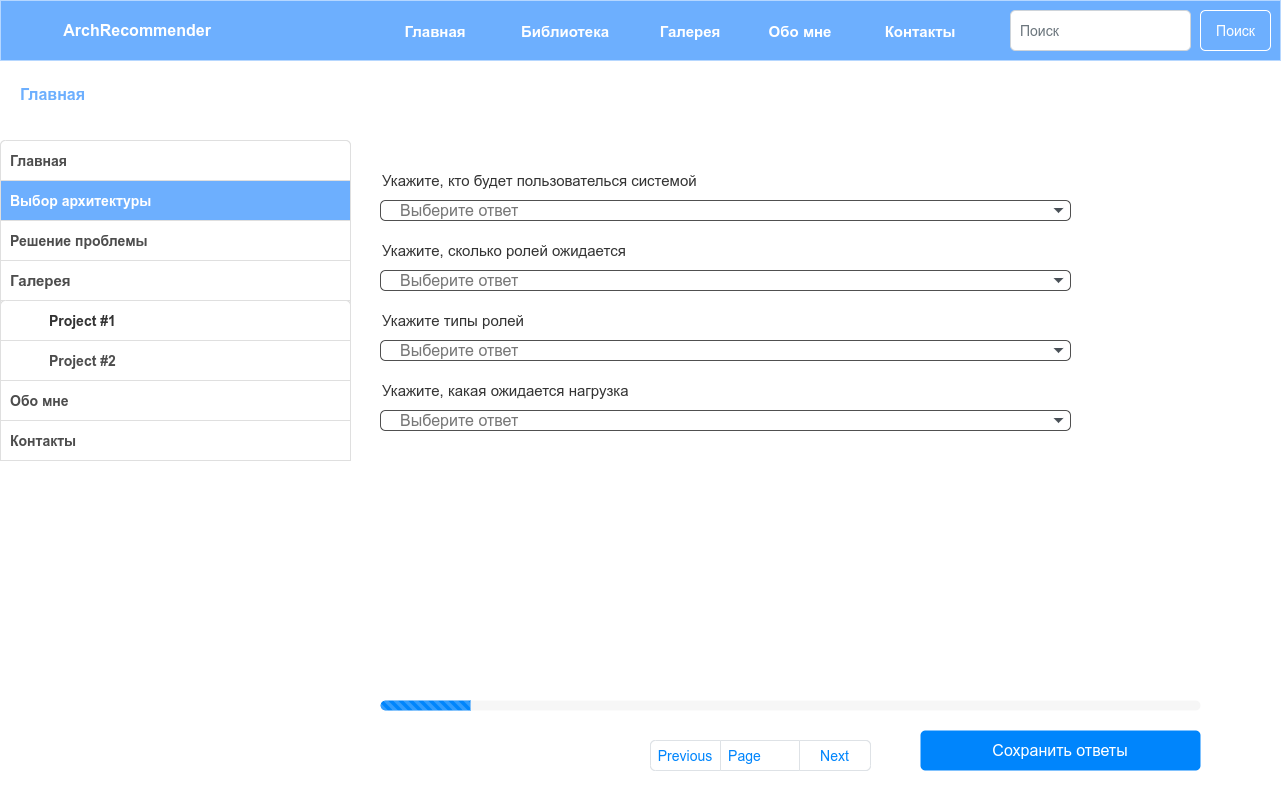
\includegraphics[scale=0.40]{Dissertation/images/DISSER-21.png}
    }
    \caption{Пользовательский ввод данных}\label{fig:ui-1}
\end{figure}

\begin{figure}[ht]
    \centerfloat{
        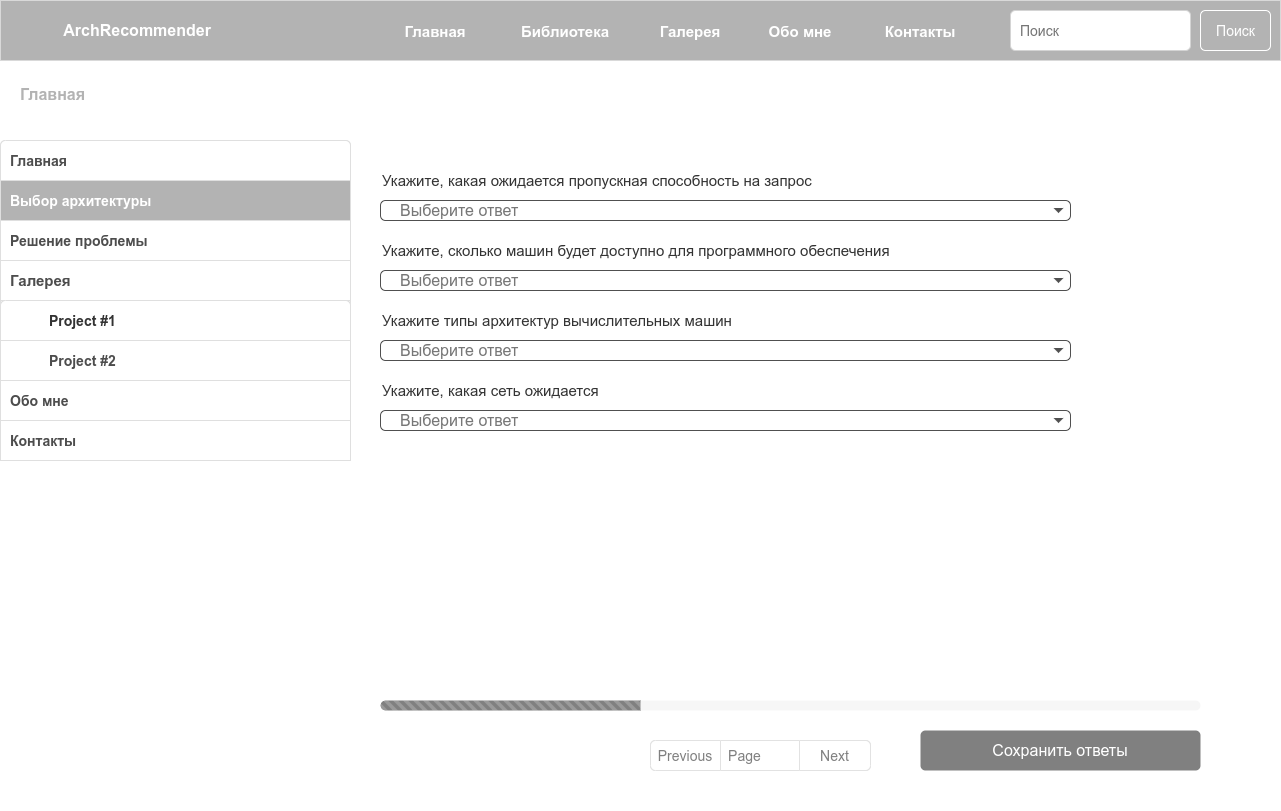
\includegraphics[scale=0.40]{Dissertation/images/DISSER-22.png}
    }
    \caption{Пользовательский ввод данных}\label{fig:ui-2}
\end{figure}

\begin{figure}[ht]
    \centerfloat{
        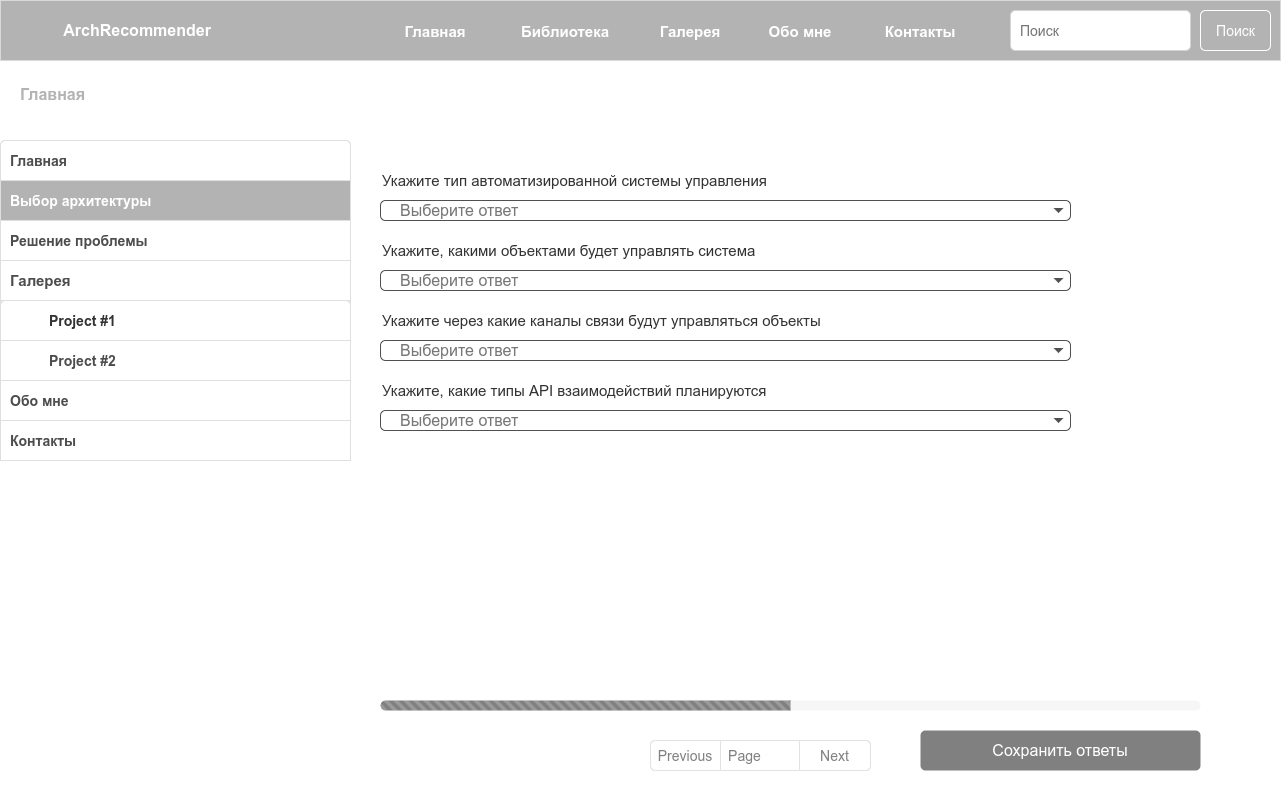
\includegraphics[scale=0.40]{Dissertation/images/DISSER-23.png}
    }
    \caption{Пользовательский ввод данных}\label{fig:ui-3}
\end{figure}

\begin{figure}[ht]
    \centerfloat{
        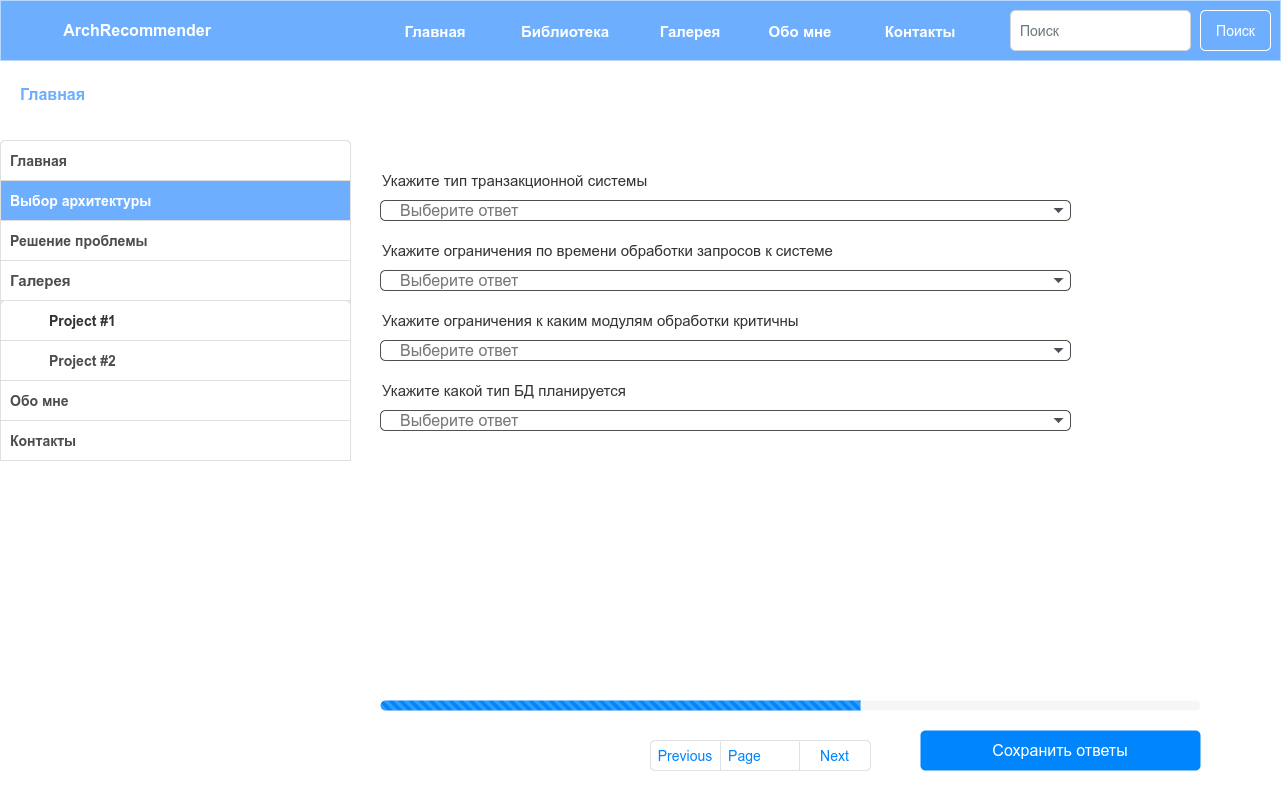
\includegraphics[scale=0.40]{Dissertation/images/DISSER-24.png}
    }
    \caption{Пользовательский ввод данных}\label{fig:ui-4}
\end{figure}

\begin{figure}[ht]
    \centerfloat{
        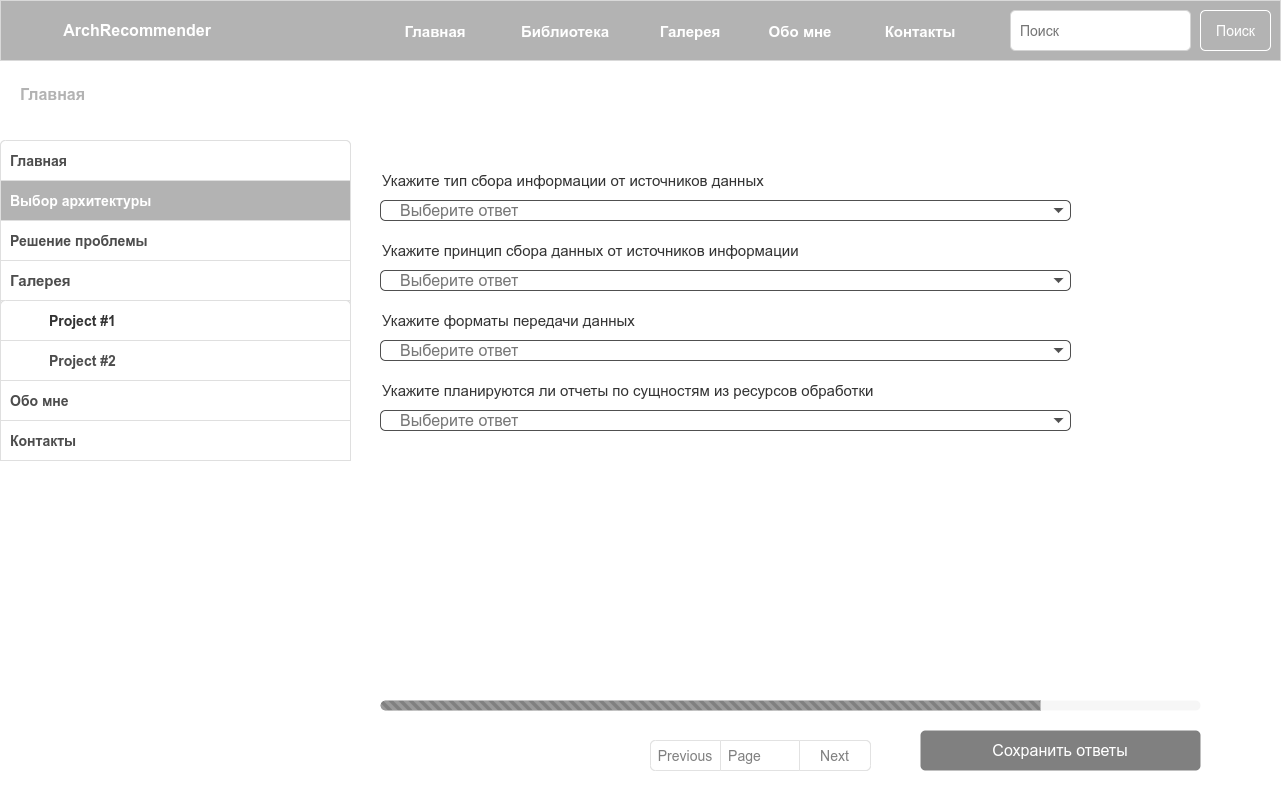
\includegraphics[scale=0.40]{Dissertation/images/DISSER-25.png}
    }
    \caption{Пользовательский ввод данных}\label{fig:ui-5}
\end{figure}

\begin{figure}[ht]
    \centerfloat{
        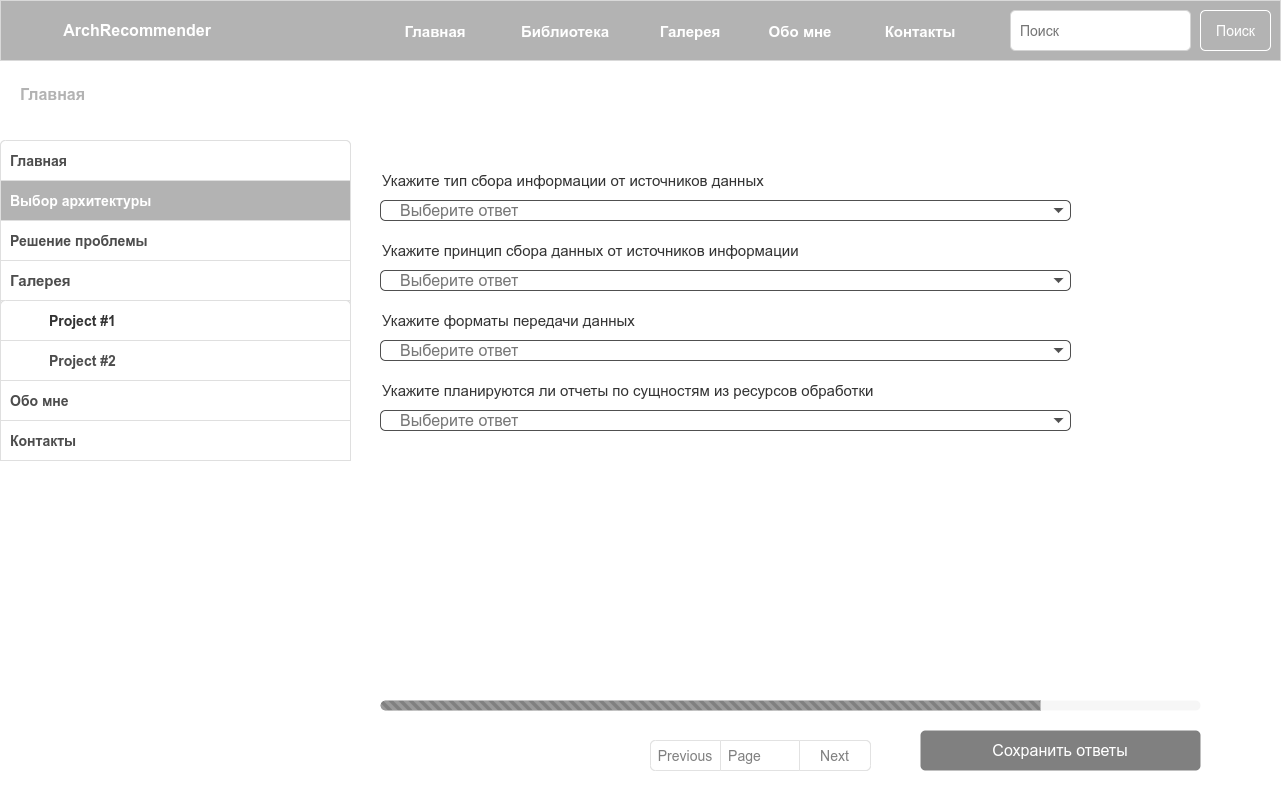
\includegraphics[scale=0.40]{Dissertation/images/DISSER-26.png}
    }
    \caption{Пользовательский ввод данных}\label{fig:ui-6}
\end{figure}


Перечень параметров указан в Таблице \cref{tab:tab_pref} приложения~\cref{app:A2}.

\subsection{Обработка данных}\label{subsec:ch3/sec3/sub2}

Обработка данных в укрупненном виде представлена на Рисунке~\cref{fig:bmodel}
\begin{figure}[ht]
    \centerfloat{
        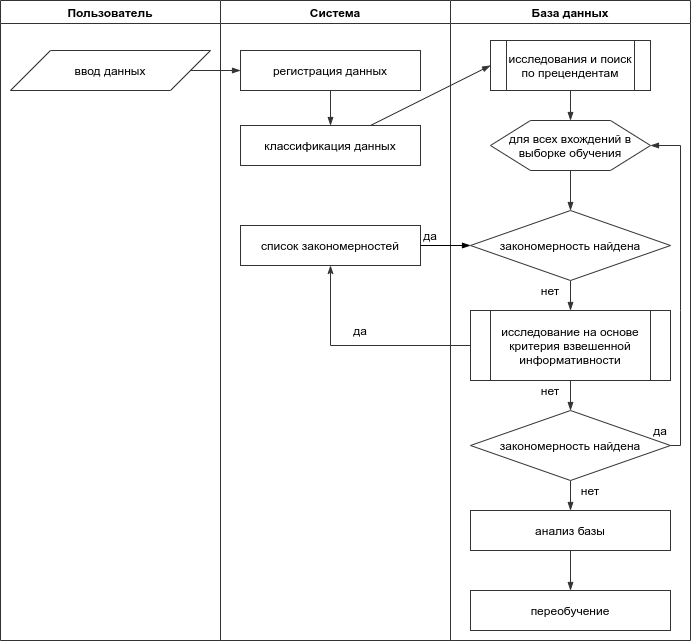
\includegraphics[scale = 0.7]{Dissertation/images/DISSER-51.png}
    }
    \caption{Обработка данных в укрупненном виде}\label{fig:bmodel}
\end{figure}



На Рисунке ~\cref{fig:FLprocess} представлен процесс обработки данных деревьев классификации на основе нечеткого вывода. 
\begin{figure}[ht]
    \centerfloat{
        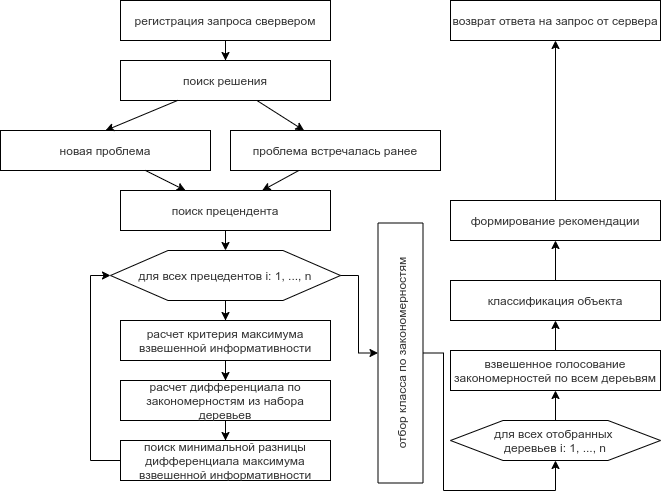
\includegraphics[scale=0.65]{Dissertation/images/DISSER-12.png}
    }
    \caption{Структура обработки информации}\label{fig:FLprocess}
\end{figure}
На Рисунке ~\cref{fig:NNprocess1} представлен процесс обработки данных деревьев классификации на основе нечеткого вывода. 
\begin{figure}[ht]
    \centerfloat{
        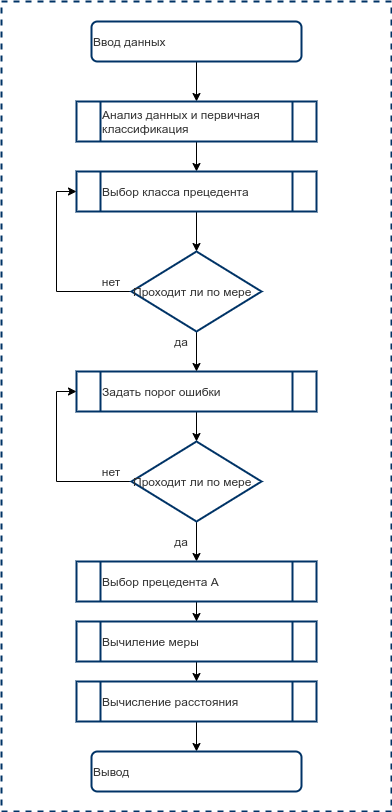
\includegraphics[scale=0.65]{Dissertation/images/DISSER-28.png}
    }
    \caption{Структура обработки информации}\label{fig:NNprocess1}
\end{figure}
На Рисунке ~\cref{fig:NNprocess2} представлен процесс обработки данных деревьев классификации на основе нечеткого вывода. 
\begin{figure}[ht]
    \centerfloat{
        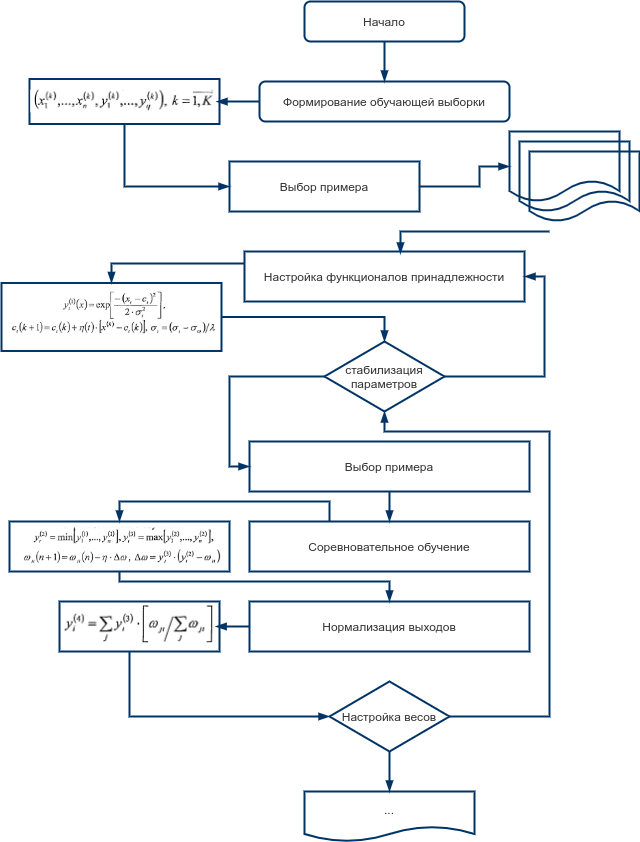
\includegraphics[scale=0.75]{Dissertation/images/DISSER-29.png}
    }
    \caption{Структура обработки информации}\label{fig:NNprocess2}
\end{figure}
На Рисунке ~\cref{fig:NNprocess3} представлен процесс обработки данных деревьев классификации на основе нечеткого вывода. 
\begin{figure}[ht]
    \centerfloat{
        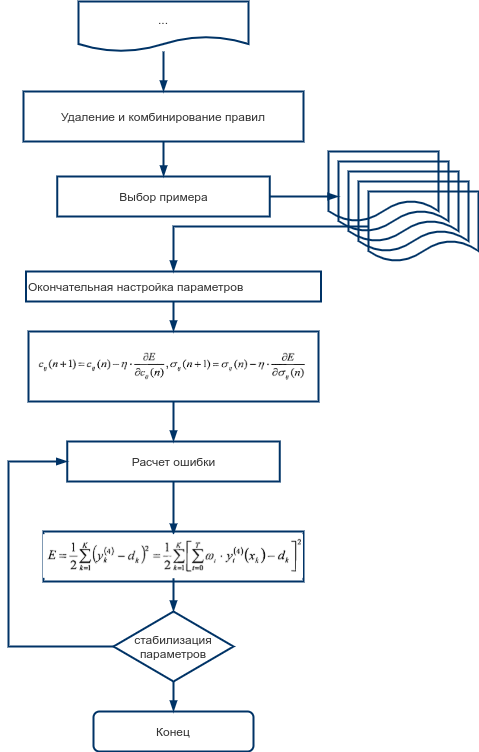
\includegraphics[scale=0.5]{Dissertation/images/DISSER-30.png}
    }
    \caption{Структура обработки информации}\label{fig:NNprocess3}
\end{figure}

\subsection{Отчеты и анализ данных}\label{subsec:ch3/sec2/sub3}
Результат работы программы представлен на Рисунке~\cref{fig:res}.
\begin{figure}[ht]
    \centerfloat{
        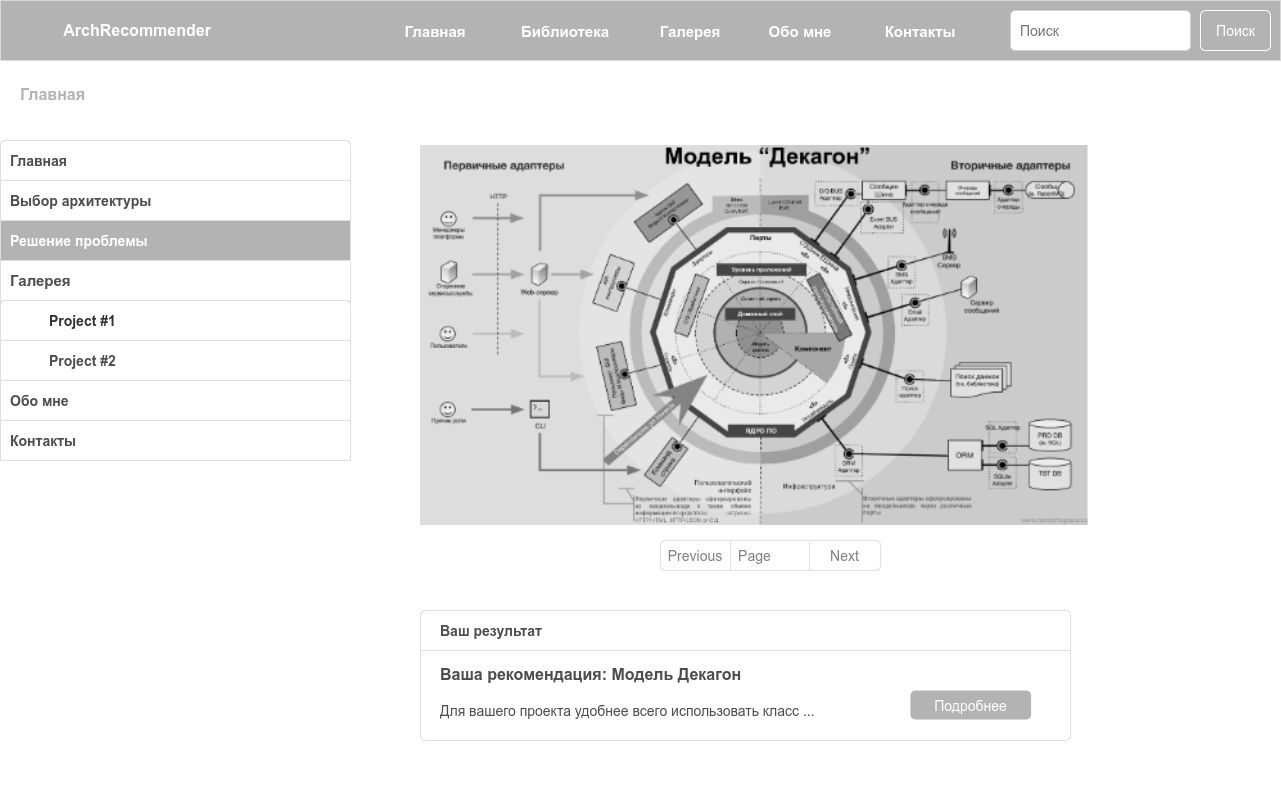
\includegraphics[scale=0.4]{Dissertation/images/DISSER-27.png}
    }
    \caption{Структура вывода информации}\label{fig:res}
\end{figure}
На Рисунке ~\cref{fig:res1} представлен результат обработки данных деревьев классификации на основе нечеткого вывода. 
\begin{figure}[ht]
    \centerfloat{
        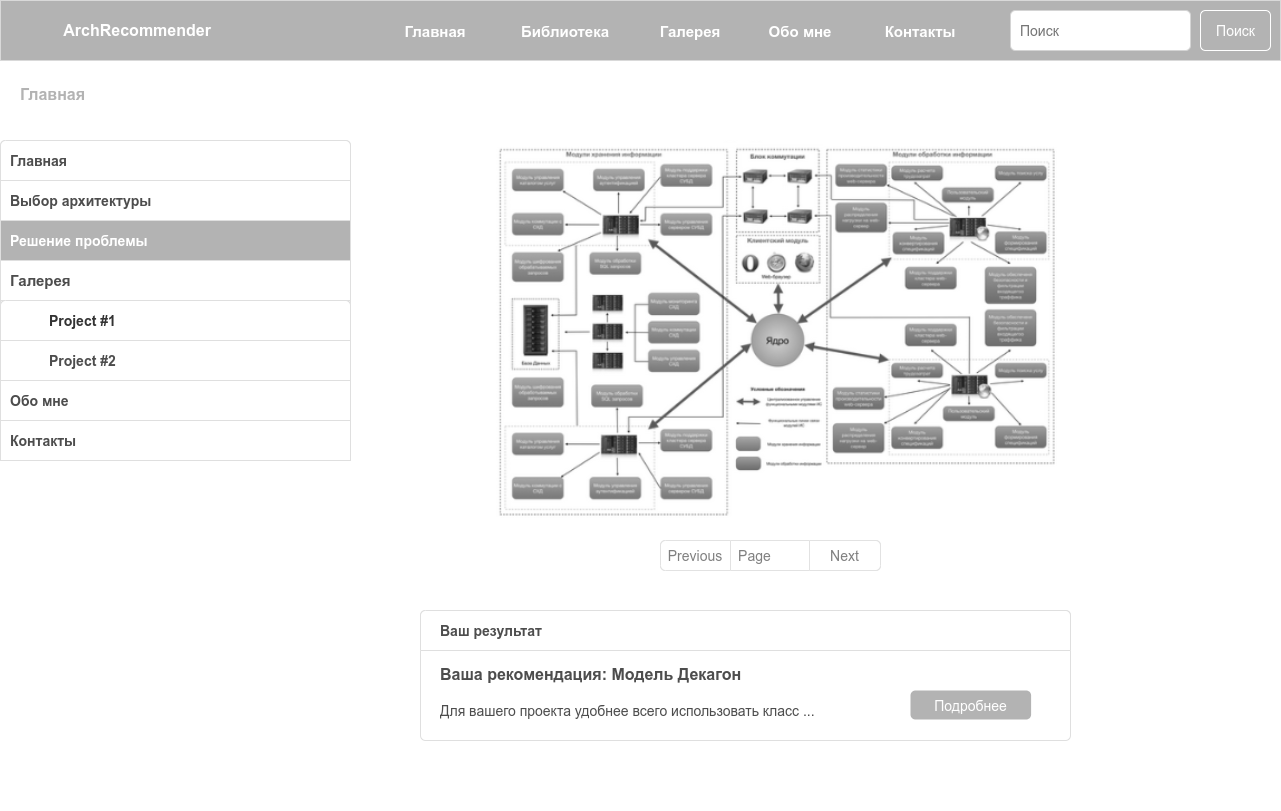
\includegraphics[scale=0.4]{Dissertation/images/DISSER-31.png}
    }
    \caption{Структура вывода информации}\label{fig:res1}
\end{figure}

\subsection{Алгоритм оценки надежности разработанного специального математического и алгоритмического обеспечения}\label{sec:ch3/sec3/sub1}

Разработанная модель специального математического и алгоритмического обеспечения для задач автоматизации процесса поддержки принятий решений относительно разработки архитектуры программного обеспечения отвечает параметрам надежности согласно следующим критериям оценки:
\begin{enumerate}
    \item энтропийный критерий.
\end{enumerate}

Рассмотрим энтропийный критерий надежности относительно модели поддержки принятий решений. Объект представляется, как система поддержки принятий решений, которая взаимодействует с окружающими ее объектами и физическим миром. Данное взаимодействие может быть представлено с помощью веществ и энергий, которые в процессе взаимодействия с объектом вызывают изменеия состояний. При таких изменениях происходят изменения состояний параметров и переменных работы самого объекта, в процесс взаимодействия объекта со средой воздействия. Такие изменения влияют на равновесие, стационарность обработки информации, стационарность работы объекта, необратимость процессов, работоспособность, могут приводить к возникновению отказов. Рассмотрим процесс изменений состояний информации в системе с точки зрения информационной энтропии процессов.
Пусть выражение
\begin{equation}
    \label{eq:equation61}
     H = -\sum_{i=1}^n{P_ilogP_i}
\end{equation}

описывает величину неопределенности в информационном потоке сообщений.

Пусть, выражение
\begin{equation}
    \label{eq:equation62}
     \int \mathrm{\frac{\partial S}{\partial t}}\,\mathrm{d}\tau
\end{equation}

описывает принцип возрастания энтропии в потоке и будет преобразовано к виду и описывает изменение энтропии в системе.
\begin{equation}
    \label{eq:equation63}
     -\frac{\partial(\rho S)}{\partial t} + \biguptriangle (\rho S v) = \theta
\end{equation}

Рассмотри задачу оценки надежности с точки зрения задачи оценки максимума производства энтропии, где основным принципом является феномен диссипации энергии в термодинамических системах. Изменения состояния в системе представим в иде классической модели марковских процессов и уравнений Колмогорова. Данная система дифференциальных уравнений представляет изменения состояния объекта, как некоторый неоднородный марковский процесс чистого размножения с дискретным числом состояний и непрерывным временем

\begin{equation}
    \label{eq:equation64}
     \left\{\begin{array}{ll} 
    \frac{dP_1(t)}{dt} = - \lambda(t)_1 P_1(t) 
    \\ \frac{dP_i(t)}{dt} = - \lambda(t)_{i-1} P_{i-1}(t) - \lambda(t)_i P_i(t)
    \\...
    \\ \frac{dP_n(t)}{dt} = -\lambda(t)_{n-1} P_{n-1}(t)
     \forall{t} \geq t_0
      & \end{array} \right. \]
\end{equation}

где  $P_1(0) = 1, P_i(0) = 0, i \in \{2,3,...,n\}$.

Уравнение энтропии  для такой системы примет следующий вид
\begin{equation}
    \label{eq:equation62}
     H(t)_k = - \int_0^t \mathrm{P_k(t)log(P_k(t))}\,\mathrm{d}t
\end{equation}

где $P_k(t)$ - вероятность отказа в $k$-м состоянии в момент времени $t$.


\subsection{Общие принципы организации сбора статистических данных по отказам и сбоям}\label{sec:ch3/sec3/sub2}

Основным общим принципом организации сбора статистических данных будет введение экспоненциальной пороговой функции потерь.  Пусть в модели уже построено $T$ закономерностей, вместе составляющих алгоритм классификации $a_{T}(x)$ ~\cite{eq:equation49, eq:equation50}.

\begin{equation}
    \label{eq:equation49}
    m = min_{x \in S_{\varepsilon}}\omega_1(x)
\end{equation}

\begin{equation}
    \label{eq:equation50}
    V(x,t) \geq \omega_1(x) \geq m
\end{equation}

В случае добавления еще одного голоса функция примет вид:
\begin{equation}
    \label{eq:equation5-1}
    \Gamma'_c(x) = \Gamma_c(x) + \alpha\phi_c(x) 
\end{equation}

Определим условие, когда алгоритм $a_{T+1}(x)$ допускает минимальное число ошибок на обучающей выборке $X^l$. 
Количство ошибок, которое алгоритм $a_{T+1}(x)$ допускает перед добавлением закономерности \phi_c:

\begin{equation}
    \label{eq:equation5-2}
        Q_T = \sum_{i=1}^{l} [\Gamma_{y_i}(x_i) - \Gamma_{y_i}(x_i) < 0]
\end{equation}

Количество ошибок, которое алгоритм $a_{T+1}(x)$ допускает после добавления закономерности \phi_c:

\begin{equation}
    \label{eq:equation5-3}
    \begin{multlined}
   Q_T = \sum_{i=1}^{l} [y_i=c][\Gamma_{y_i}(x_i) - \Gamma_{y_i}(x_i) + 
     \alpha\phi_c(x_i) < 0] + \\
     + [y_c \neq 0] [\Gamma_{y_i}(x_i) - \Gamma_{y_i}(x_i) 
     - \alpha\phi_c(x_i) < 0] 
     \end{multlined}
\end{equation}

Вышеприведенный функционал является разрывной функцией т.к. содержит параметр \alpha следующего вида $[z(\alpha)<0]$. Минимизация этого функционала  является комбинаторной задачей оптимизации нетривиального вида. Такую задачу будем рассматривать приближенно и заменим пороговую функцию непрерывно дифференцируемой оценкой сверху $[z < 0] \leq e^{-z}$:

\begin{equation}
    \label{eq:equation5-4}
   Q_T \leq \tilde{Q}_T \equiv \sum_{i=1}^{l}e^{\Gamma_{-y_i}(x_i) - \Gamma_{y_i}(x_i)}} = \sum_{i=1}^{l}\omega_{i}
\end{equation}

В случае, если алгоритм верно классифицирует объект $x_{i}$, то $\omega_{i} < 1$. Если алгоритм ошибается, то $\omega_{i} > 1$. Чем больше перевес в пользу ошибочного класса, тем больше вес $\omega_{i}$. 



\section{Выводы по главе}\label{sec:ch3/conc}
В результате проведенной работы в данной главе были решены следующие задачи:
\begin{enumerate}
    \item проанализированы проблемы процесса обработки информации, 
    \item продемонстрирован механизм сбора информации, проведена организация сбора информации от пользователя о системе, планируемой к проектированию,
    \item определены структура, состав и характеристика входных наборов переменных, для которых составляется рекомендация,
    \item продемонстрирована алгоритмическая реализация процесса сбора, обработки информации, процесса параметризации внутреннего механизма создания рекомендаций,
    \item продемонстрирована алгоритмическая структура реализации работы нейронной сети на основе нечеткого вывода.
\end{enumerate}

В данной главе предоставлено описание пользовательского интерфейса и структуры ввода и вывода информации. Систему поддержки принятия решений следует дополнить функционалом более детального анализа по качеству отношений между сущностями. Также следует разработать механизм классификации иерархии классов в проекте.

\clearpage
